\begin{frame}{Experiments on link prediction}

  \begin{itemize}
    \item Link prediction on a graph dataset: given a graph with some edges removed, predict the likelihood
    for each pair of nodes to be connected by an edge
    \item Cora dataset \cite{McCallum_2000}: 2708 publications, 5429 links, 1433-dimensional feature vectors
    \item Using a Variational Graph Auto-Encoder \cite{kipf_variational_2016}: a variational encoder which uses a
    graph neural network (GNN) as encoder
    \item Reconstruction loss:
        $$ \mathbb{E}_{q(\mathbf{Z}|\mathbf{X}, \mathbf{A})}(\log p(\mathbf{A}|\mathbf{Z})) \quad 
        \text{where} \quad p(\mathbf{A}|\mathbf{Z}) = \prod_{i = 1}^N \prod_{j=1}^N p(A_{i, j}|\mathbf{z}_i, \mathbf{z}_j) $$
    \item Negative sampling: in the sum $\sum_{i, j} \log p(A_{i, j}|\mathbf{z}_i, \mathbf{z}_j)$, keep all
    positive edges and one randomly sampled negative edge per positive edge
  \end{itemize}
\end{frame}


\begin{frame}{Loss computation}

  \begin{itemize}
    \item[$\blacksquare$] Reconstruction loss
      \begin{itemize}
        \item $$\mathcal{L}_{recon} =  - \mathbb{E}_{q_{\psi}}( log\ p_{\phi}(x | z)) $$
        \item$$ -\nabla_{\kappa} \mathcal{L}_{recon} \approx g_{recon} + g_{cor} $$ 
      \end{itemize}
    \item[$\blacksquare$] KL Divergence 
        \begin{itemize}
          \item $$ \mathcal{L}_{\mathcal{KL}} = \mathcal{KL}(q(z|\mu, \kappa) || p(z)) $$
          \item $$ \nabla_{\kappa} \mathcal{L}_{\mathcal{KL}} $$
        \end{itemize}
  \end{itemize}
  The formulas were explicity computed in the article.
  
\end{frame}

\begin{frame}{Training curves for $\mathcal{N}$-VGAE}
  Latent dimension $16$, learning rate $0.01$. No KL divergence in loss.
  \begin{center}
    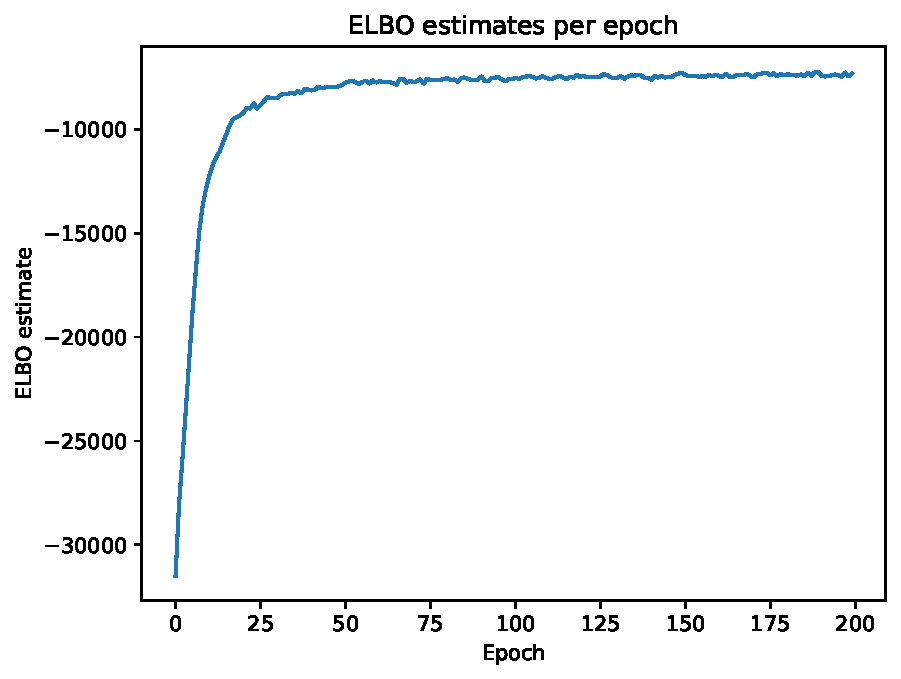
\includegraphics[width=.8\hsize]{figures/normal_elbo_estimates.pdf}
  \end{center}
\end{frame}

\begin{frame}{Area under ROC curve for $\mathcal{N}$-VGAE}
  \begin{center}
    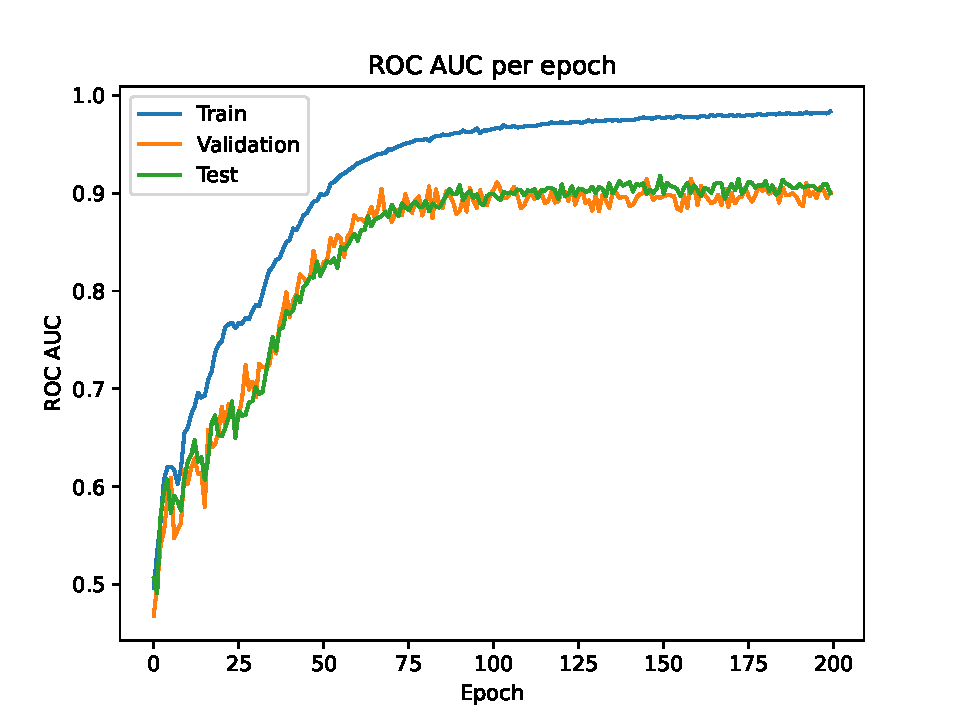
\includegraphics[width=.8\hsize]{figures/normal_auc.pdf}
  \end{center}
\end{frame}

\begin{frame}{Average precision for $\mathcal{N}$-VGAE}
  \begin{center}
    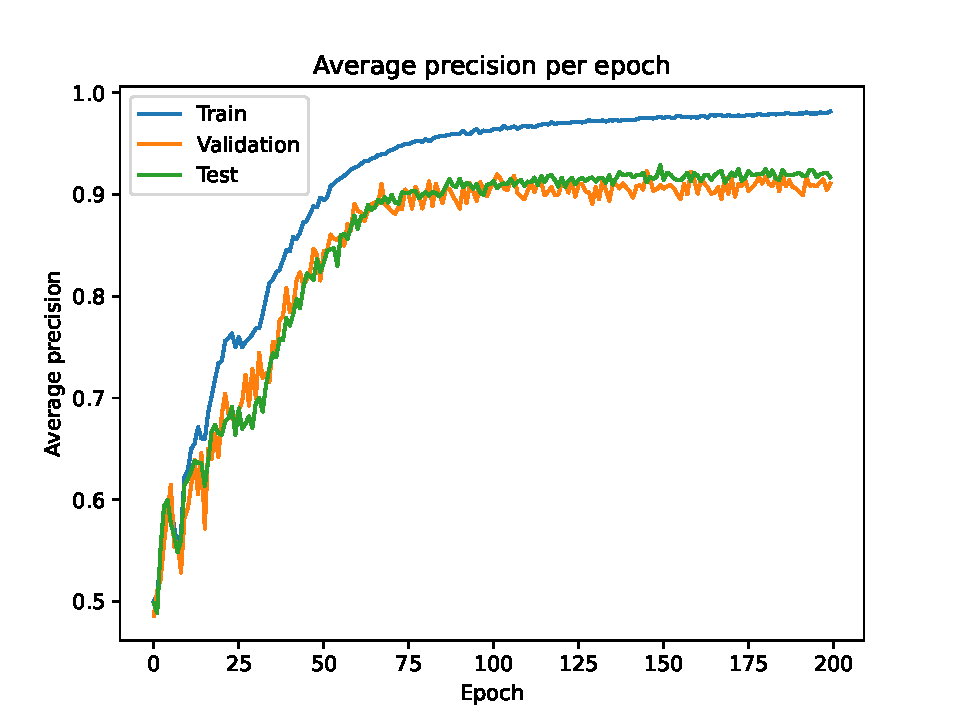
\includegraphics[width=.8\hsize]{figures/normal_ap.pdf}
  \end{center}
\end{frame}

\begin{frame}{Training curves for $\mathcal{S}$-VGAE}
  Latent dimension $16$, learning rate $0.01$. No KL divergence in loss.
  \begin{center}
    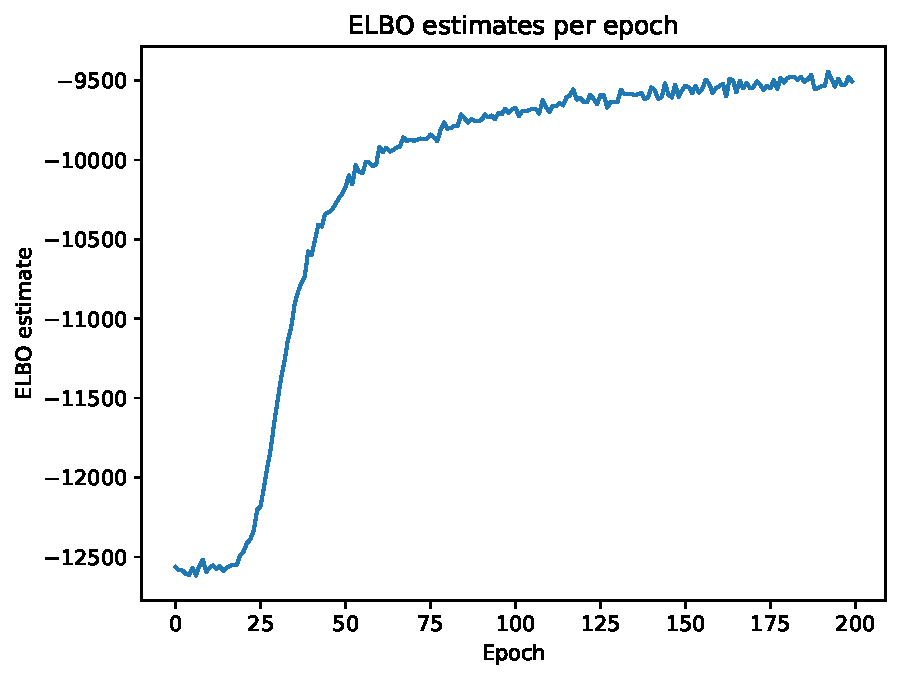
\includegraphics[width=.8\hsize]{figures/vMF_elbo_estimates.pdf}
  \end{center}
\end{frame}

\begin{frame}{Area under ROC curve for $\mathcal{S}$-VGAE}
  \begin{center}
    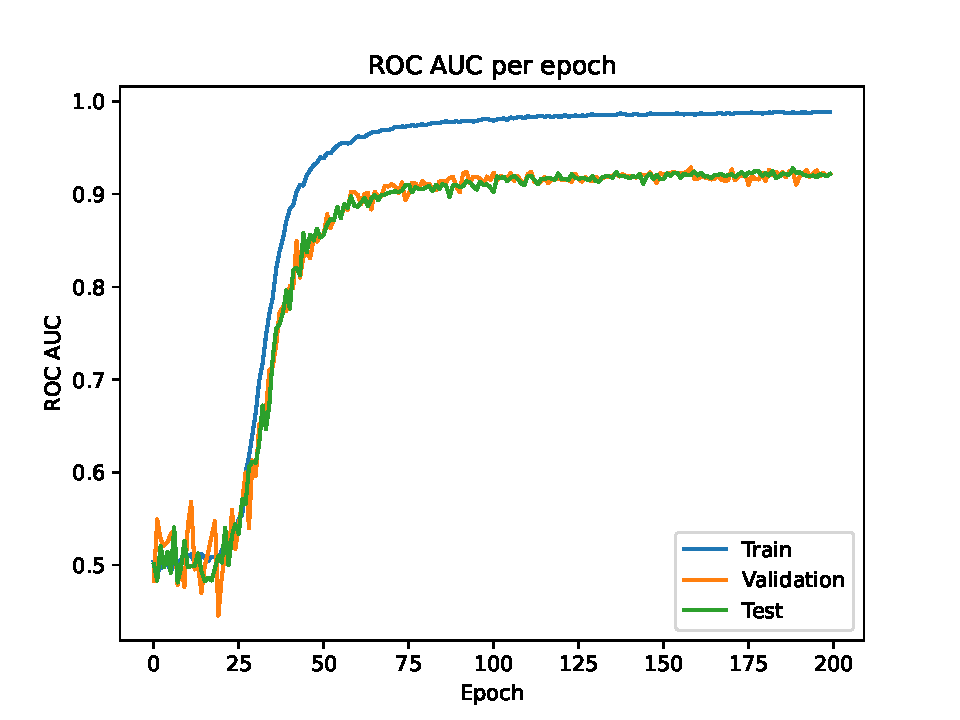
\includegraphics[width=.8\hsize]{figures/vMF_auc.pdf}
  \end{center}
\end{frame}

\begin{frame}{Average precision for $\mathcal{S}$-VGAE}
  \begin{center}
    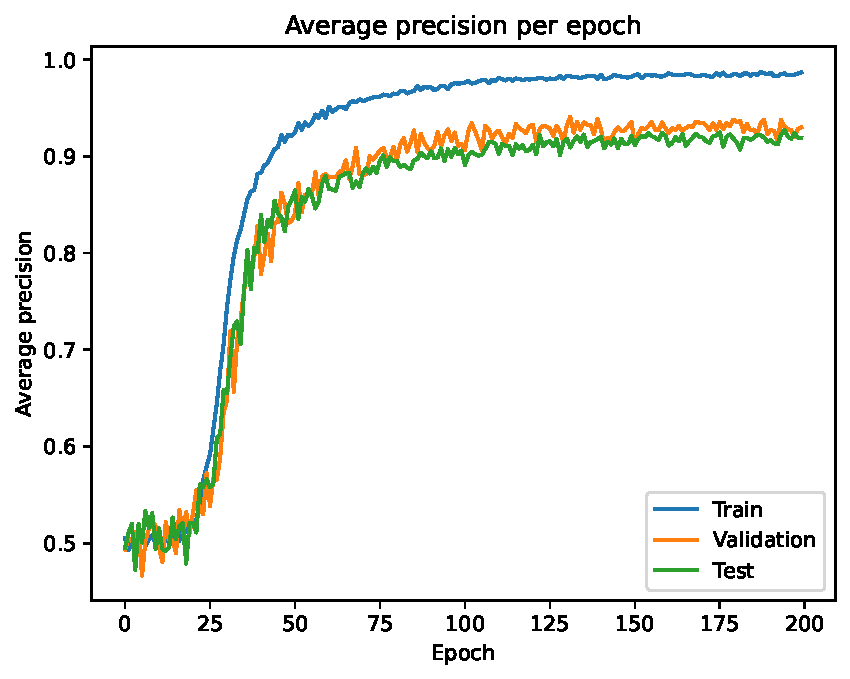
\includegraphics[width=.8\hsize]{figures/vMF_ap.pdf}
  \end{center}
\end{frame}

\begin{frame}{Impact of dimension $d$ on $\mathcal{S}$-VGAE}
  \centering
  vmf d8 : mean auc : 0.90, 0.004638416275088545 \\
  vmd d8 : mean ap : 0.90, 0.006861910798200132 \\
  vmf d16 : mean auc : 0.91, 0.005106467210129149 \\
  vmd d16 : mean ap : 0.91, 0.002400819600884836 \\
  vmf d32 : mean auc : 0.92, 0.003988671804848861 \\
  vmd d32 : mean ap : 0.92, 0.006771540977322898 \\
  vmf d64 : mean auc : 0.92, 0.004086768956130232 \\
  vmd d64 : mean ap : 0.92, 0.006337561094050328 \\
\end{frame}